\documentclass[fleqn]{article}
\usepackage[a4paper,
mag=1000, includefoot,
left=2.5cm, right=1cm, top=2cm, bottom=2cm,
headsep=0.7cm, footskip=1cm]{geometry}
\usepackage{mathtext}
\usepackage{parskip}
\usepackage{setspace}
\linespread{1.2}

\usepackage[most]{tcolorbox}

\usepackage{amsmath,amssymb,amsthm,amscd,amsfonts}
\usepackage{cmap}
\usepackage[utf8]{inputenc}
\usepackage[T2A]{fontenc}
\usepackage[russian]{babel}
\usepackage{hyperref}
\hypersetup{
	colorlinks=true,
	linkcolor=blue,
	filecolor=magenta,      
	urlcolor=cyan,
	pdftitle={Overleaf Example},
	pdfpagemode=FullScreen,
}

\usepackage{euscript}
\usepackage{mathdots}
\usepackage{graphicx}
\usepackage[russian]{cleveref}
\usepackage{epstopdf}

\newcommand{\sn}{\mathrm{sn}\,}
\newcommand{\am}{\mathrm{am}\,}
\newcommand{\cn}{\mathrm{cn}\,}
\newcommand{\dn}{\mathrm{dn}\,}

\title{Эллиптический интеграл}

\begin{document}
	
	\maketitle
	\hrule
	Материал из Википедии --- свободная энциклопедия
	\begin{tcolorbox}[colback=cyan!5!white,colframe=black]
	\centering{Текущая версия страницы пока не проверялась опытными участниками и может ссылаться на \cite{miln-tomson, korn1984, Beitman1967, Achiyezer1970, matlab}}
	\end{tcolorbox}
	
	\emph{Эллипт\'{и}ческий интегр\'{а}л} --- некоторая функция $f$ над полем действительных или комплексных чисел, которая может быть формально представлена в следующем виде:
	\begin{equation}\label{eq:1} f(x)=\int^x_cR(t,P(t))\,dt.\end{equation}
	где $R$ — рациональная функция двух аргументов из \eqref{eq:1}, $P$ — квадратный корень из многочлена 3-й или 4-й степени, не имеющего кратных корней, $c$ — некоторая константа из поля, где определена функция.
	
	В общем случае эллиптический интеграл не может быть формально выражен в элементарных функциях. Исключением являются случаи, когда $P$ имеет кратные корни или когда многочлены в $R(x, y)$ не содержат нечётных степеней $y$.
	
	Однако для каждого эллиптического интеграла существуют формулы приведения его к сумме элементарных функций и от одного до трёх нормальных эллиптических интегралов, называемых эллиптическими интегралами 1-го, 2-го и 3-го рода).
	
	\tableofcontents
	
	\section{История} 
	\hrule
	В интегральном исчислении эллиптический интеграл появился в связи с задачей вычисления длины дуги эллипса и был впервые исследован Джулио Фаньяно, а позднее — Леонардом Эйлером.
	\section{Обозначения}
	\hrule
	Эллиптические интегралы часто представляют в виде функции ряда различных аргументов. Эти различные аргументы полностью эквивалентны (они дают одни и те же интегралы), но может возникнуть путаница, связанная с их различным происхождением. В большинстве работ авторы придерживаются канонического наименования. Прежде чем определить сами интегралы, необходимо ввести наименования для аргументов:
	\begin{itemize}
		\item $\alpha$ --- \emph{модулярный угол} (иногда модулярный угол обозначается лигатурой \oe);
		\item $k = \sin{\alpha}$ --- \emph{модуль эллиптического интеграла};
		\item $m=k^2=\sin^2{\alpha}$ --- \emph{параметр}.
	\end{itemize}
	
	Следует отметить, что нормальные эллиптические интегралы Лежандра, как полные, так и неполные, являются чётными функциями модуля $k$ (и модулярного угла $\alpha$). Их область определения $-1 \leqslant k \leqslant +1$.
	
	Иногда, преимущественно в советской научной литературе, под параметром эллиптического интеграла подразумевают характеристику нормального эллиптического интеграла Лежандра 3-го рода (напр., Корн Г., Корн Т. «Справочник по математике для научных работников и инженеров»).
	
	Заметим, что представленные выше величины определяются одна через другую; определение одной из них задаёт и две остальные.
	
	Эллиптический интеграл зависит также и от другого параметра, который, как и предыдущий, можно ввести несколькими способами:
	\begin{itemize}
		\item $x=\sin{\varphi}=\sn u$, где $\sn$ --- \emph{эллиптическая функция Якоби};
		\item $\varphi = \arcsin{x} = \am u$ --- \emph{амплитуда};
	\end{itemize}
	Определение одного из этих параметров определяет остальные. Таким образом, они могут использоваться вперемешку. Заметим, что $u$ зависит также и от $m$. Несколько дополнительных уравнений связывают $u$ с другими параметрами:
	\begin{equation*}\cos{\varphi}=\cn u\end{equation*}
	и
	\begin{equation}\sqrt{1 - m \sin^2{\varphi}}=\dn u\label{eq:2} \end{equation}
	Последнее иногда называется в \eqref{eq:2} \emph{дельта амплитуда} и записывается как
	\begin{equation*}\Delta (\varphi) = \dn u.\end{equation*}
	Иногда в литературе ссылаются на \textit{дополнительный параметр}, \textit{дополнительный модуль} или \textit{дополнительный модулярный угол}. Их вводят следующим способом:
	\begin{itemize}
		\item $m_1=1-m$ --- \emph{дополнительный параметр};
		\item $k' = \sqrt{1 - k^2}$ --- \emph{дополнительный модуль};
		\item $k'^2=m_1$ --- \emph{дополнительный модулярный угол}.
	\end{itemize}
	\section{Нормальный эллиптический интеграл 1-го рода (неполный)}
	\hrule
	\emph{Нормальный эллиптический интеграл Лежандра 1-го рода} $F$ определяется как
	\begin{equation*}F(\varphi, k) = \int^\varphi_0\frac{d\theta}{\sqrt{1-k^2\sin^2{\theta}}}\end{equation*}
	или, в форме Якоби,
	\begin{equation*}F(x, k)=\int_0^x\frac{dz}{\sqrt{(1-z^2)(1-k^2z^2)}}.\end{equation*}
	
	Обозначения эллиптических интегралов не являются универсально общепринятыми. Следует различать такие разделители между переменной и параметром, как «\textbackslash», «|» и «,». Там, где в качестве разделителя используется вертикальная черта, за ней ставится параметр интеграла, тогда как за обратной косой чертой ставится модулярный угол. В частности, верно соотношение.
	\begin{equation*}F(\varphi, \sin{\alpha}=F(\varphi|sin^2{\alpha}=F(\varphi \backslash \alpha))).\end{equation*}
	\subsection{Частные случаи}
	\begin{align*}
		F&(\varphi \backslash 0)=\varphi; \\
		F&(i\varphi \backslash 0) = i\varphi; \\
		F&(\varphi \backslash 90^\circ) = \ln{(\sec{\varphi} + \tg{\varphi})}=\ln\,\tg(\frac{\pi}{4}+\frac{\varphi}{2}); \\
		F&(i\varphi \backslash 90^\circ) = i\,\arctg{(\sh{\varphi})};
	\end{align*}
	\section{Нормальный эллиптический интеграл 2-го рода (неполный)}
	\hrule
	\emph{Нормальный эллиптический интеграл Лежандра 2-го рода} $E$ определяется как
	\begin{equation*}E(\varphi, k)=\int_0^\varphi \sqrt{1-k^2\sin^2 \theta}\, d\theta,\end{equation*}
	или, используя подстановку $x = \sin \varphi$, перейдём к \eqref{eq:3}
	\begin{equation*}E(x, k)=\int_0^x\frac{\sqrt{1-k^2z^2}}{\sqrt{1-z^2}}\, dz.\end{equation*}
	\subsection{Частные случаи}
	\begin{align}
		E&(\varphi, 0) = \varphi; \label{eq:3}\\
		E&(i\varphi, 0) = i\varphi; \nonumber\\
		E&(\varphi, 1) = \sin \varphi; \nonumber\\
		E&(i\varphi, 1) = i \sh \varphi; \nonumber
	\end{align}
	\section{Нормальный эллиптический интеграл 3-го рода (неполный)}
	\hrule
	\emph{Нормальный эллиптический интеграл Лежандра 3-го рода} $\Pi$ определяется как
	\begin{equation*}\Pi(c;\varphi, k)=\int_0^\varphi \frac{d\theta}{(1+c\sin^2\theta)\sqrt{1-k^2\sin^2\theta}}\end{equation*}
	или
	\begin{equation*}\Pi(c;x,k)=\int_0^x\frac{dx}{(1+cx^2)\sqrt{(1-k^2x^2)(1-x^2)}}.\end{equation*}
	Число $c$ называется \emph{характеристикой} и может принимать любое значение, независимо от остальных аргументов. Свойства эллиптического интеграла 3-го рода существенно зависят от величины характеристики. Заметим, что значение интеграла $Pi(-1;\pi/2|m)$ стремится к бесконечности для любых $m$.
	\subsection{Гиперболический случай}
	\subsubsection{$\mathbf{(0<c<m)}$}
	Введём дополнительные обозначения:
	\begin{align*}
		\varepsilon& = \arcsin\sqrt{\frac{n}{sin^2\alpha}},\qquad 0\leqslant\varepsilon\leqslant\frac{\pi}{2}; \\
		\beta& = \frac{\pi\,F(\varepsilon \backslash 90^\circ - \alpha)}{2K(\alpha)}; \\
		q&=q(\alpha); \\
		\nu&=\frac{\pi\,F(\varphi\backslash\alpha)}{2K(\alpha)}; \\
		\delta_2&=\sqrt{\frac{c}{(1-c)(c-\sin^2\alpha)}};\\
		K&(\alpha) - \text{полный нормальный эллиптический интеграл Лежандра 1-го рода.}
	\end{align*}
	Тогда можно записать интеграл через тета-функции Якоби:
	\begin{equation*}\Pi(c;\;\varphi \setminus \alpha )=\delta _{1}\left(-{\frac {1}{2}}\,\ln {\frac {\vartheta _{4}(\nu +\beta )}{\vartheta _{4}(\nu -\beta )}}+\nu \,{\frac {\vartheta _{1}'(\beta )}{\vartheta _{1}(\beta )}}\right),\end{equation*}
	где
	\begin{equation*}\frac{1}{2}\,\ln\frac{\vartheta_4(\nu+\beta)}{\vartheta_4(\nu-\beta)} = 2 \sum_{s=1}^{\infty} \frac{q^s}{s(1-q^{2s})}\sin{2s\nu}\,\sin\,{2s\beta}\end{equation*}
	и
	\begin{equation*}{\frac {\vartheta _{1}'(\beta )}{\vartheta _{1}(\beta )}}=\operatorname {ctg} \,\beta +4\sum _{s=1}^{\infty }{\frac {q^{2s}}{1-2q^{2s}\cos {2\beta }+q^{4s}}}\sin {2\beta }.\end{equation*}
	\subsubsection{$\mathbf{(c>1)}$}
	С помощью подстановки $C = \frac{\sin^2\alpha}{c}$ этот случай сводится к предыдущему, так как $0<C<sin^2\alpha$. Введём дополнительно величину 
	\begin{equation*}p_1={\sqrt{(c-1)\left(1-{\frac{\sin^2\alpha }{c}}\right)}}.\end{equation*}
	Тогда:
	\begin{equation*}\Pi (c;\;\varphi\setminus\alpha )=-\Pi (C;\;\varphi \setminus \alpha )+F(\varphi\setminus\alpha)+\frac {1}{2p_1}\ln \left({\frac {\Delta (\varphi )+p_1\tg \,\varphi}{\Delta(\varphi )-p_1\tg\,\varphi}}\right).\end{equation*}
	\subsection{Круговой случай}
	\subsubsection{$\mathbf{(m<c<1)}$}
	Введём дополнительные обозначения:
	\begin{align*}
		\varepsilon& = \arcsin\sqrt{\frac{1-n}{\cos^2\alpha}}, \qquad 0\leqslant\varepsilon\leqslant\frac{\pi}{2}; \\
		\beta& = \frac{\pi\,F(\varepsilon\backslash 90^\circ - \alpha)}{2K(\alpha)}; \\
		q&=q(\alpha); \\
		\nu& = \frac{\pi F(\varphi\backslash\alpha)}{2K(\alpha)}; \\
		\delta_2&=\sqrt{\frac{c}{(1-c)(c-\sin^2\alpha)}}.
	\end{align*}
	Тогда эллиптический интеграл равен:
	\begin{equation*}\Pi(c;\varphi\backslash\alpha)=\delta_2(\lambda-4\mu\nu),\end{equation*}
	где
	\begin{equation*}\lambda = \arctg(\th\beta\tg\nu)+ 2\sum_{s=1}^\infty \frac{(-1)^{s-1}}{s}\frac{q^{2s}}{1-q^{2s}}\sin{2s\nu}\,\sh\,{2s\beta}\end{equation*}
	и
	\begin{equation*}\mu ={\dfrac {\sum \limits _{s=1}^{\infty }sq^{s^{2}}\,\operatorname {sh} \,{2s\beta }}{1+\sum \limits _{s=1}^{\infty }q^{s^{2}}\,\operatorname {ch} \,{2s\beta }}}.\end{equation*}
	\subsubsection{$\mathbf{(c<0)}$}
	С помощью подстановки $C = \frac{\sin^2\alpha-c}{1-c}$ этот случай сводится к предыдущему, так как $\sin^2\alpha < C < 1.$ Введём дополнительную величину
	\begin{equation*}p_2=\sqrt{\frac{ -c(\sin^2\alpha-c)}{1-c}}.\end{equation*}
	Тогда:
	\begin{multline*}{
			\sqrt {(1-c)\left(1-{\frac {\sin ^{2}\alpha }{c}}\right)}}\,\Pi (c;\;\varphi \setminus \alpha )=
		\\ {\sqrt {(1-C)\left(1-{\frac {\sin ^{2}\alpha }{C}}\right)}}\,\Pi (C;\;\varphi \setminus \alpha )\,
		\\ +\,{\frac {\sin ^{2}\alpha \,F(\varphi \setminus \alpha )}{p_{2}}}\,
		\\ +\, \arctg \,\left({\frac {p_{2}}{2}}{\frac {\sin {2\varphi }}{\Delta (\varphi )}}\right).
		\\ \end{multline*}
	\section{Полный нормальный эллиптический интеграл Лежандра 1-го рода}
	\hrule
	\begin{figure}[h]
	\centering
	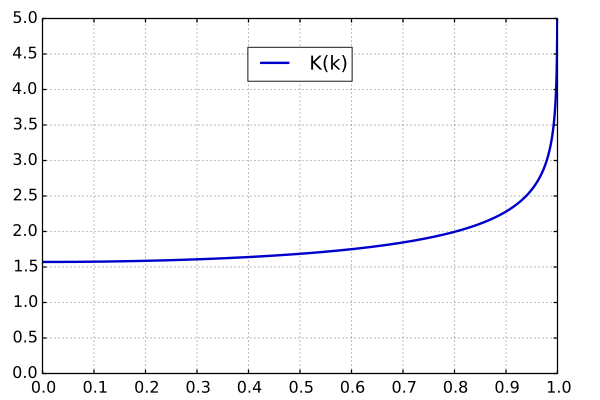
\includegraphics[width=0.8\textwidth]{Graphs/FirstKk.png}
	\caption{Параболический график}
	\label{fig:parabolic graph}
	\end{figure}
	В случае, если амплитуда $\varphi$ нормального эллиптического интеграла Лежандра 1-го рода (пример выше \eqref{fig:parabolic graph}) равна $\pi/2$, он называется \textit{полным} нормальным эллиптическим интегралом Лежандра 1-го рода: 
	\begin{equation*}K(k)=\int_0^{\pi/2}\frac{d\varphi}{\sqrt{1-k^2\sin^2\varphi}}=F(\pi/2,k)\end{equation*}
	или
	\begin{equation*}K(k)=\int^1_0\frac{dx}{\sqrt{(1-x^2)(1-k^2x^2)}}.\end{equation*}
	Полный эллиптический интеграл 1-го рода можно представить в виде степенного ряда:
	\begin{equation*}K(k)={\frac {\pi }{2}}\sum _{n=0}^{\infty }\left({\frac {(2n)!}{2^{2n}n!^{2}}}\right)^{2}k^{2n},\end{equation*}
	что эквивалентно выражению
	\begin{equation*}K(k)={\frac {\pi }{2}}\left(1+\left({\frac {1}{2}}\right)^{2}k^{2}+\left({\frac {1\cdot 3}{2\cdot 4}}\right)^{2}k^{4}+\ldots +\left({\frac {(2n-1)!!}{(2n)!!}}\right)^{2}k^{2n}+\ldots \right),\end{equation*}
	где $n!!$ обозначает двойной факториал.
	
	Полный эллиптический интеграл 1-го рода можно записать через гипергеометрическую функцию следующим образом:
	\begin{equation*}K(k)={\frac {\pi }{2}}\,_{2}F_{1}\left({\frac {1}{2}},\;{\frac {1}{2}};\;1;\;k^{2}\right).\end{equation*}
	\subsection{Частные случаи}
	\begin{align*}
		K&(0)=\frac{\pi}{2}.\\
		K&(1)=\infty. \\
		K&\left({\frac {\sqrt {2}}{2}}\right)={\frac {\Gamma \left({\frac {1}{4}}\right)^{2}}{4{\sqrt {\pi }}}}. \\
		K&\left({\frac {{\sqrt {6}}-{\sqrt {2}}}{4}}\right)={\frac {2^{-{\frac {7}{3}}}3^{\frac {1}{4}}\Gamma \left({\frac {1}{3}}\right)^{3}}{\pi }}. \\ 
		K&\left({\frac {{\sqrt {6}}+{\sqrt {2}}}{4}}\right)={\frac {2^{-{\frac {7}{3}}}3^{\frac {3}{4}}\Gamma \left({\frac {1}{3}}\right)^{3}}{\pi }}. \\
		\sn& \,K=\sin {\frac {\pi }{2}}=1. \\
		\cn& \,K=\cos {\frac {\pi }{2}}=0. \\
		\dn& \,K={\sqrt {1-k^{2}}}=k'.
	\end{align*}
	\subsection{Производная полного эллиптического интеграла 1-го рода}
	\begin{equation*}{\frac {\mathrm {d} K(k)}{\mathrm {d} k}}={\frac {E(k)}{k(1-k^{2})}}-{\frac {K(k)}{k}},\end{equation*}
	где $E(k)$ --- полный нормальный эллиптический интеграл Лежандра 2-го рода, определённый в следующем разделе.
	\subsection{Дифференциальное уравнение}
	Полный эллиптический интеграл 1-го рода является решением дифференциального уравнения
	\begin{equation*}{\frac {d}{dk}}\left(k\left(1-k^{2}\right){\frac {dK(k)}{dk}}\right)=kK(k).\end{equation*}
	Вторым решением этого уравнения является
	\begin{equation*}K\left(\sqrt{1-k^2}\right).\end{equation*}
	\section{Полный нормальный эллиптический интеграл Лежандра 2-го рода}
	\hrule
	\begin{figure}[h]
		\centering
		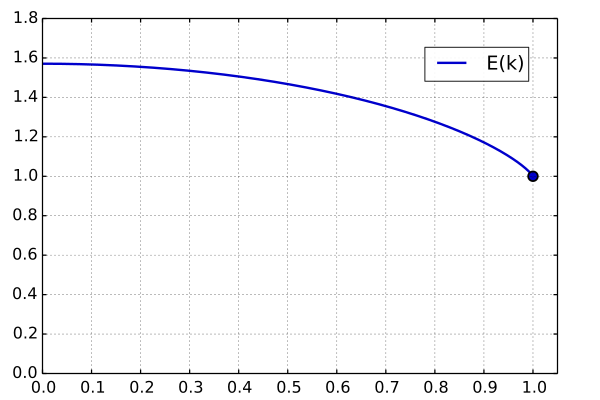
\includegraphics[width=0.8\textwidth]{Graphs/SecondEk.png}
		\caption{ПНЭИ Лежандра 2-го рода}
		\label{fig: FNEI Second}
	\end{figure}
	В случае, если амплитуда $\varphi$ нормального эллиптического интеграла Лежандра 2-го рода равна $\pi/2$, он называется полным нормальным эллиптическим интегралом Лежандра 2-го рода, как график выше (\eqref{fig: FNEI Second}):
	 \begin{equation*}E(k)=\int \limits _{0}^{\pi /2}\!{\sqrt {1-k^{2}\sin ^{2}\varphi }}\,d\varphi =E(\pi /2,\;k)\end{equation*}
	 или
	 \begin{equation*}E(k) = \int \limits_{0}^{1}\,\frac{\sqrt{1-k^2 x^2}}{\sqrt{1-x^2}}\,dx.\end{equation*}
	 Полный эллиптический интеграл 2-го рода можно представить в виде степенного ряда (см. \eqref{eq:4}, \eqref{eq:3}):
	 \begin{equation*}E(k)={\frac {\pi }{2}}\sum _{n=0}^{\infty }\left({\frac {(2n)!}{2^{2n}n!^{2}}}\right)^{2}{\frac {k^{2n}}{1-2n}},\end{equation*}
	 что эквивалентно выражению 
	 \begin{equation*}E(k)={\frac {\pi }{2}}\left(1-\left({\frac {1}{2}}\right)^{2}{\frac {k^{2}}{1}}-\left({\frac {1\cdot 3}{2\cdot 4}}\right)^{2}{\frac {k^{4}}{3}}-\ldots -\left({\frac {(2n-1)!!}{(2n)!!}}\right)^{2}{\frac {k^{2n}}{2n-1}}-\ldots \right).\end{equation*}
	 Полный эллиптический интеграл 2-го рода можно записать через гипергеометрическую функцию следующим образом:
	 \begin{equation*}E(k)={\frac {\pi }{2}}\,_{2}F_{1}\left({\frac {1}{2}},\;-{\frac {1}{2}};\;1;\;k^{2}\right).\end{equation*}
	\subsection{Частные случаи}
	\begin{align}
		E&(0)=\frac{\pi}{2}. \nonumber \\
		E&(1)=1. \nonumber \\
		E&\left({\frac {\sqrt {2}}{2}}\right)=\pi ^{\frac {3}{2}}\Gamma \left({\frac {1}{4}}\right)^{-2}+{\frac {\Gamma \left({\frac {1}{4}}\right)^{2}}{8{\sqrt {\pi }}}}. \nonumber \\
		E&\left({\frac {{\sqrt {6}}-{\sqrt {2}}}{4}}\right)=2^{\frac {1}{3}}3^{-{\frac {3}{4}}}\pi ^{2}\Gamma \left({\frac {1}{3}}\right)^{-3}+2^{-{\frac {10}{3}}}3^{-{\frac {1}{4}}}{\frac {{\sqrt {3}}+1}{\pi }}\Gamma \left({\frac {1}{3}}\right)^{3}. \label{eq:4}\\
		E&\left({\frac {{\sqrt {6}}+{\sqrt {2}}}{4}}\right)=2^{\frac {1}{3}}3^{-{\frac {1}{4}}}\pi ^{2}\Gamma \left({\frac {1}{3}}\right)^{-3}+2^{-{\frac {10}{3}}}3^{\frac {1}{4}}{\frac {{\sqrt {3}}-1}{\pi }}\Gamma \left({\frac {1}{3}}\right)^{3}. \nonumber
	\end{align}
	\subsection{Производная полного эллиптического интеграла 2-го рода}
	\begin{equation*}{\frac {\mathrm {d} E(k)}{\mathrm {d} k}}={\frac {E(k)-K(k)}{k}}.\end{equation*}
	\subsection{Дифференциальное уравнение}
	Полный эллиптический интеграл 2-го рода является решением дифференциального уравнения
	\begin{equation*}\left(k^{2}-1\right){\frac {d}{dk}}\left(k\;{\frac {dE(k)}{dk}}\right)=kE(k).\end{equation*}
	Вторым решением этого уравнения является функция $E\left(\sqrt{1-k^2}\right)-K\left(\sqrt{1-k^2}\right).$
	\section{Полный нормальный эллиптический интеграл Лежандра 3-го рода}
	\hrule
	\begin{figure}[h]
		\centering
	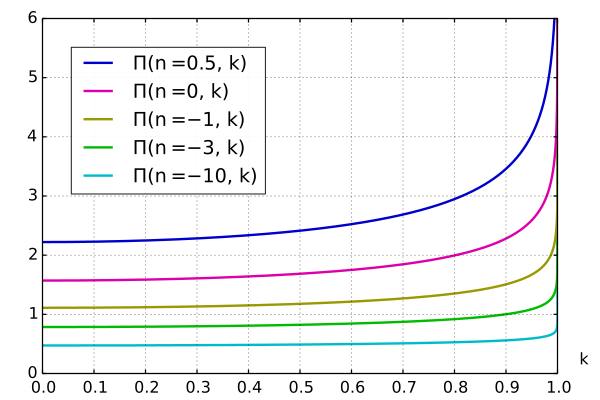
\includegraphics[width=0.8\textwidth]{Graphs/ThirdMulti.png}
	\caption{Графики ПНЭИ Лежандра 3-го рода}
	\label{fig: FNEI Third}
	\end{figure}
	Аналогично полным эллиптическим интегралам 1-го и 2-го рода можно ввести полный эллиптический интеграл 3-го рода как в \eqref{fig: FNEI Third}:
	\begin{equation*}\Pi (c,\;k)=\Pi (c;\;\pi /2,\;k)=\int \limits _{0}^{\pi /2}\!{\frac {d\varphi }{(1+c\sin ^{2}\varphi ){\sqrt {1-k^{2}\sin ^{2}\varphi }}}}.\end{equation*}
	или
	\begin{equation*}\Pi (c,\;k)=\Pi (c;\;1,\;k)=\int \limits _{0}^{1}\!{\frac {dx}{(1+cx^{2}){\sqrt {(1-k^{2}x^{2})(1-x^{2})}}}}.\end{equation*}
	\subsection{Гиперболический случай}
	\subsubsection{$\mathbf{(0<c<m)}$}
	\begin{equation*}\Pi(c \setminus \alpha) = K(\alpha) + \delta_1K(\alpha)Z(\varepsilon \setminus \alpha).\end{equation*}
	где $Z(\varepsilon\backslash\alpha)$ --- дзета-функция Якоби.
	\subsubsection{$\mathbf{(c>1)}$}
	\begin{equation*}\Pi (c\setminus \alpha )=K(\alpha )-\Pi (C\setminus \alpha ).\end{equation*}
	\subsection{Круговой случай}
	\subsubsection{$\mathbf{(m<c<1)}$}
	\begin{equation*}\Pi (c\setminus \alpha )=K(\alpha )+{\frac {1}{2}}\pi \delta _{2}\left(1-\Lambda _{0}(\varepsilon \setminus \alpha )\right),\end{equation*}
	где $\Lambda_0(\varepsilon\backslash\alpha)$ --- лямбда-функция Хеймана.
	\subsubsection{$\mathbf{(c<0)}$}
	\begin{equation*}\Pi (c\setminus \alpha )=-{\frac {c\cos ^{2}\alpha \,\Pi (C\setminus \alpha )}{(1-c)(\sin ^{2}\alpha -n)}}+{\frac {\sin ^{2}\alpha }{\sin ^{2}\alpha -c}}K(\alpha ).\end{equation*}
	\subsection{Частные производные}
	\begin{align*}{\frac {\partial \Pi (c,k)}{\partial c}}&={\frac {1}{2\left(k^{2}-c\right)(c-1)}}\left(E(k)+{\frac {1}{c}}\left(k^{2}-c\right)K(k)+{\frac {1}{c}}\left(c^{2}-k^{2}\right)\Pi (c,k)\right).\\
	{\frac {\partial \Pi (c,k)}{\partial k}}&={\frac {k}{c-k^{2}}}\left({\frac {E(k)}{k^{2}-1}}+\Pi (c,k)\right).
	\end{align*}
	\section{Дополнительные эллиптические интегралы (неполные)}
	\hrule
	\subsection{Дзета-функция Якоби}
	\begin{equation*}Z(\varphi \setminus \alpha )=E(\varphi \setminus \alpha )-{\frac {E(\alpha )F(\varphi \setminus \alpha )}{K(\alpha )}}.\end{equation*}
	\subsection{Лямбда-функция Хеймана}
	\begin{equation*}\Lambda _{0}(\varphi \setminus \alpha )={\frac {F(\varphi \setminus 90^{\circ }-\alpha )}{K'(\alpha )}}+{\frac {2}{\pi }}K(\alpha )\,Z(\varphi \setminus 90^{\circ }-\alpha ).\end{equation*}
	или
	\begin{equation*}\Lambda _{0}(\varphi \setminus \alpha )={\frac {2}{\pi }}\left(K(\alpha )\,E(\varphi \setminus 90^{\circ }-\alpha )-\left(K(\alpha )-E(\alpha )\right)\,F(\varphi \setminus 90^{\circ }-\alpha )\right).\end{equation*}
	\section{См. также}
	\hrule
	\begin{itemize}
		\item \href{/wiki/%D0%AD%D0%BB%D0%BB%D0%B8%D0%BF%D1%82%D0%B8%D1%87%D0%B5%D1%81%D0%BA%D0%B8%D0%B5_%D1%84%D1%83%D0%BD%D0%BA%D1%86%D0%B8%D0%B8}{Эллиптические функции}
		\item \href{/wiki/%D0%AD%D0%BB%D0%BB%D0%B8%D0%BF%D1%82%D0%B8%D1%87%D0%B5%D1%81%D0%BA%D0%B0%D1%8F_%D0%BA%D1%80%D0%B8%D0%B2%D0%B0%D1%8F}{Эллиптическая кривая}
		\item \href{/wiki/%D0%A1%D0%BF%D0%B5%D1%86%D0%B8%D0%B0%D0%BB%D1%8C%D0%BD%D1%8B%D0%B5_%D1%84%D1%83%D0%BD%D0%BA%D1%86%D0%B8%D0%B8}{Специальные функции}
		\item \href{/wiki/%D0%90%D0%BF%D0%BF%D1%80%D0%BE%D0%BA%D1%81%D0%B8%D0%BC%D0%B0%D1%86%D0%B8%D0%B8_%D1%8D%D0%BB%D0%BB%D0%B8%D0%BF%D1%82%D0%B8%D1%87%D0%B5%D1%81%D0%BA%D0%B8%D1%85_%D0%B8%D0%BD%D1%82%D0%B5%D0%B3%D1%80%D0%B0%D0%BB%D0%BE%D0%B2}{Аппроксимация эллиптических интегралов}
	\end{itemize}
	
	\hrule
%	\begin{itemize}
%		\item \textit{Бобылёв Д. К.} Эллиптические интегралы и функции // Энциклопедический словарь Брокгауза и Ефрона : в 86 т. (82 т. и 4 доп.). — СПб., 1890—1907.
%	\end{itemize}
%	\section{Ссылки}
%	\hrule
%	\begin{itemize}
%		\item \textit{Милн-Томсон Л.} Эллиптические интегралы // Справочник по специальным функциям с формулами, графиками и таблицами / Под ред. М. Абрамовица и И. Стиган; пер. с англ. под ред. В. А. Диткина и Л. Н. Карамзиной. — М.: Наука, 1979. — С. 401—441. — 832 с. — 50 000 экз.
%		\item \textit{Корн Г., Корн Т.} Справочник по математике для научных работников и инженеров. — М.: Наука, 1977.
%		\item \textit{Бейтмен Г. Эрдейи А.} Высшие трансцендентные функции. — Т. 3 (гл. 13).
%		\item \textit{Ахиезер Н. И.} Элементы теории эллиптических функций. (гл. 3, 7).
%		\item Эллиптические функции, Процедуры для Matlab.
%	\end{itemize}
	
	
	\bibliographystyle{ugost2008}
	\bibliography{EI_reference}
\end{document}